\chapter{Machine learning}\label{chap13}

Machine learning (ML) approaches are often characterized by high-dimensional parameter spaces, which are implicit in non-parametric inference. It is important to note that non-parametric inference refers to models with potentially infinite parameters, not the absence of parameters. This is known as the wide problem, where the number of features, and consequently parameters, can exceed the sample size. Another common challenge in ML is the tall problem, which arises when the sample size is extremely large. In such cases, scalable algorithms are required.

\section{Cross validation and Bayes factors}\label{sec13_1}
Prediction is central in machine learning, particularly in supervised learning. Therefore, the starting point is a set of ``raw'' regressors \( \mathbf{W} \), which are used to construct a set of features \( \mathbf{w} = T(\mathbf{W}) \), where \( T(\cdot) \) denotes a \textit{dictionary of transformations} such as polynomials, interactions between variables, application of functions like exponentials, and so on. These features are then used to predict $y$ through a model $f(\mathbf{w})$,
\begin{align*}
	y_i &= f(\mathbf{w}_i) + \mu_i,
\end{align*}
where $\mu_i \stackrel{\text{i.i.d.}}{\sim} (0, \sigma^2)$.

We predict \( y \) using \( \hat{f}(\mathbf{w}) \), a model trained on the data. Thus, the expected squared error (ESE) at a fixed set of features, taking into account that \( \mathbb{E}_{\mathcal{D},\boldsymbol{\mu}} \left[\mu_i(f(\mathbf{w}_i) - \hat{f}(\mathbf{w}))\right] = 0 \) by independence, and defining \( \bar{f}(\mathbf{w}_i) = \mathbb{E}_{\mathcal{D}}[\hat{f}(\mathbf{w}_i)] \), is given by:

\begin{align*}
	\text{ESE} &= \mathbb{E}_{\mathcal{D},y} \left[ (y - \hat{f}(\mathbf{w}))^2 \right] \\
	&= \mathbb{E}_{\mathcal{D},\boldsymbol{\mu}} \left[ \left(f(\mathbf{w}_i) + \mu_i - \hat{f}(\mathbf{w})\right)^2 \right] \\
	&= \mathbb{E}_{\mathcal{D},\boldsymbol{\mu}} \left[ (f(\mathbf{w}_i) - \hat{f}(\mathbf{w}))^2 + 2\mu_i(f(\mathbf{w}_i) - \hat{f}(\mathbf{w})) + \mu_i^2 \right] \\
	&= \mathbb{E}_{\mathcal{D}} \left[ (f(\mathbf{w}_i) - \hat{f}(\mathbf{w}))^2 \right] + \mathbb{E}_{\boldsymbol{\mu}} \left[ \mu_i^2 \right] \\
	&= \mathbb{E}_{\mathcal{D}} \left[ \left((f(\mathbf{w}_i) - \bar{f}(\mathbf{w}_i)) - (\hat{f}(\mathbf{w}) - \bar{f}(\mathbf{w}_i)) \right)^2 \right] + \sigma^2 \\
	&= \underbrace{\mathbb{E}_{\mathcal{D}} \left[ (f(\mathbf{w}_i) - \bar{f}(\mathbf{w}_i))^2 \right]}_{\text{Bias}^2} + \underbrace{\mathbb{E}_{\mathcal{D}} \left[ (\hat{f}(\mathbf{w}) - \bar{f}(\mathbf{w}_i))^2 \right]}_{\text{Variance}} + \underbrace{\sigma^2}_{\text{Irreducible Error}}.
\end{align*}
Thus, the ESE is composed of the squared bias, the variance of the prediction (which is a random variable due to data variation $\mathcal{D}$), and the irreducible error. The key insight is that increasing model complexity, such as by including more features, typically reduces bias but increases variance. This trade-off can lead to overfitting, where models perform well on the training data but poorly on new, unseen data. There is, therefore, an optimal point at which the predictive error is minimized (see Figure~\ref{fig:bias_var}).\footnote{However, recent developments show that powerful modern machine learning methods, such as deep neural networks, often overfit and yet generalize remarkably well on unseen data. This phenomenon is known as \textit{double descent} or \textit{benign overfitting} \cite{belkin2019reconciling, bartlett2020benign, hastie2022surprises}.}

\begin{figure}[h!]
	\centering
	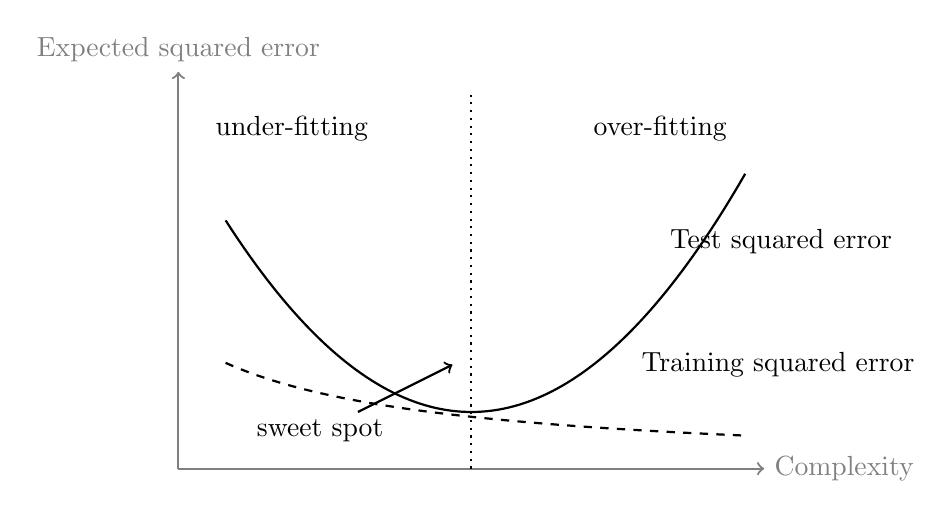
\begin{tikzpicture}[scale=1.2]
		% Axes
		\draw[->, thick, gray] (0,0) -- (6.2,0) node[right] {Complexity};
		\draw[->, thick, gray] (0,0) -- (0,4.2) node[above] {Expected squared error};
		
		% Labels for under-fitting and over-fitting
		\node at (1.2,3.6) {under-fitting};
		\node at (5.1,3.6) {over-fitting};
		
		% Training risk curve
		\draw[thick, dashed, domain=0.5:6, samples=100] plot(\x, {1.4/(0.5*\x + 1)});
		\node[right] at (4.8,1.1) {Training squared error};
		
		% Test risk curve
		\draw[thick, domain=0.5:6, samples=100] plot(\x, {0.3*(\x - 3.1)^2 + 0.6});
		\node[right] at (5.1,2.4) {Test squared error};
		
		% Sweet spot annotation
		\draw[->, thick] (1.9,0.6) -- (2.9,1.1);
		\node[align=center] at (1.5,0.4) {sweet spot};
		
		% Vertical line at optimal capacity
		\draw[dotted, thick] (3.1,0) -- (3.1,4);
		
	\end{tikzpicture}
\begin{tablenotes}
	\item \small{\textbf{Notes:} Curves for training squared error (dashed line) and test squared error (solid line). The classical U-shaped error curve arising from the bias–variance trade-off.}
\end{tablenotes}
\caption{\textit{Bias-variance trade-off} in machine learning.}
\label{fig:bias_var}
\end{figure}
    
To avoid overfitting in machine learning, an important step called \textit{cross-validation} is often employed. This involves splitting the dataset into multiple parts (called \textit{folds}) and systematically training and testing models on these parts \cite{hastie2009elements,efron2021computer}. The main goal is to evaluate how well models generalize to ``unseen data''.

There is a compelling justification for cross-validation within Bayesian inference proposed by \cite{Bernardo1994} in their section 6.1.6. The point of departure is to assume an $\mathcal{M}$-open view of nature, in which there exists a set of models $\mathcal{M} = \left\{M_j : j \in J\right\}$ under comparison, but none of them represents the true data-generating process, which is assumed to be unknown. Nevertheless, we can compare the models in $\mathcal{M}$ based on their posterior risk functions (see Chapter~\ref{chap1}) without requiring the specification of a true model. In this framework, we select the model that minimizes the posterior expected loss. Unfortunately, we cannot explicitly compute this posterior expected loss due to the lack of knowledge of the true posterior distribution under the $\mathcal{M}$-open assumption.\footnote{This is not the case under an $\mathcal{M}$-closed view of nature, where one of the candidate models is assumed to be the true data-generating process. In that setting, the posterior distribution becomes a mixture distribution with mixing probabilities given by the posterior model probabilities (see Chapter~\ref{chap10}).}

Given the expected loss conditional on model \( j \) for a predictive problem, where the action \( a \) is chosen to minimize the posterior expected loss:
\begin{align*}
	\mathbb{E}_{y_0}[L(Y_0,a) \mid M_j, \mathbf{y}] &= \int_{\mathcal{Y}_0} L(y_0, a \mid M_j, \mathbf{y}) \, \pi(y_0 \mid \mathbf{y}) \, dy_0,
\end{align*}
we note that there are \( N \) possible partitions of the dataset \( \mathbf{y} = \{y_1, y_2, \dots, y_N\} \) following a leave-one-out strategy, i.e., \( \mathbf{y} = \{\mathbf{y}_{-k}, y_k\} \), for \( k = 1, \dots, N \), where \( \mathbf{y}_{-k} \) denotes the dataset excluding observation \( y_k \). Assuming that \( \mathbf{y} \) is exchangeable, meaning its joint distribution is invariant to reordering, and that \( N \) is large, then \( \mathbf{y}_{-k} \) and \( y_k \) are good proxies for \( \mathbf{y} \) and \( y_0 \), respectively. Consequently,
\begin{align*}
	\frac{1}{K} \sum_{k=1}^K L(y_k, a \mid M_j, \mathbf{y}_{-k}) 
	\stackrel{p}{\rightarrow}\int_{\mathcal{Y}_0} L(y_0, a \mid M_j, \mathbf{y}) \, \pi(y_0 \mid \mathbf{y}) \, dy_0,
\end{align*}
by the law of large numbers, as \( N \to \infty \) and \( K \to \infty \).

Thus, we can select a model by minimizing the expected squared error based on its expected predictions \( \mathbb{E}[y_k \mid M_j, \mathbf{y}_{-k}] \); that is, we select the model with the lowest value of
\[
\frac{1}{K} \sum_{k=1}^K \left( \mathbb{E}[y_k \mid M_j, \mathbf{y}_{-k}] - y_k \right)^2.
\]

Note that if we want to compare two models based on their relative predictive accuracy using the log-score function \cite{martin2022optimal}, we select model \( j \) if
\begin{align*}
	\int_{\mathcal{Y}_0} \log\frac{p(y_0 \mid M_j, \mathbf{y})}{p(y_0 \mid M_l, \mathbf{y})} \, \pi(y_0 \mid \mathbf{y}) \, dy_0 > 0.
\end{align*}
However, we know that
\begin{align*}
	\frac{1}{K}\sum_{k=1}^K\log\frac{p(y_k \mid M_j, \mathbf{y}_{-k})}{p(y_k \mid M_l, \mathbf{y}_{-k})} 
	\stackrel{p}{\rightarrow} \int_{\mathcal{Y}_0} \log\frac{p(y_0 \mid M_j, \mathbf{y})}{p(y_0 \mid M_l, \mathbf{y})} \, \pi(y_0 \mid \mathbf{y}) \, dy_0,
\end{align*}
by the law of large numbers as \( N \to \infty \) and \( K \to \infty \).

This implies that we select model \( j \) over model \( l \) if
\begin{align*}
	\prod_{k=1}^K \left( \frac{p(y_k \mid M_j, \mathbf{y}_{-k})}{p(y_k \mid M_l, \mathbf{y}_{-k})} \right)^{1/K} 
	= \prod_{k=1}^K \left( B_{jl}(y_k, \mathbf{y}_{-k}) \right)^{1/K} > 1,
\end{align*}
where \( B_{jl}(y_k, \mathbf{y}_{-k}) \) is the Bayes factor comparing model \( j \) to model \( l \), based on the posterior \( \pi(\boldsymbol{\theta}_m \mid M_m, \mathbf{y}_{-k}) \) and the predictive \( \pi(y_k \mid \boldsymbol{\theta}_m) \), for \( m \in \{j, l\} \).

Thus, under the log-score function, cross-validation reduces to the geometric average of Bayes factors that evaluate predictive performance based on the leave-one-out samples \( \mathbf{y}_{-k} \).

\section{Regularization}\label{sec13_2}

In this century, the amount of available data continues to grow. This means we have access to more covariates for prediction, and we can also generate additional features to enhance the predictive power of our models. As a result, we often encounter \textit{wide} datasets, where the number of features may exceed the number of observations. Even in modest settings, we might have hundreds of features, and we can use them to identify which ones contribute to accurate predictions. However, we generally avoid using all features at once due to the risk of overfitting. Thus, we require a class of feature selection or \textit{regularization}.

In the Frequentist inferential framework, there has been extensive development of techniques aimed at regularization. These include methods such as Ridge regression \cite{hoerl1970ridge}, discrete subset selection techniques like best subset selection \cite{furnival1974regressions}, and forward and backward stepwise selection \cite{hastie2009elements}, as well as continuous subset selection methods such as the LASSO \cite{tibshirani1996regression}, the elastic net \cite{zou2005regularization}, and OSCAR \cite{bondell2008simultaneous}. 

It is important to note, however, that Ridge regression does not perform variable selection; rather, it shrinks coefficient estimates toward zero without setting them exactly to zero.

Ridge regression and the LASSO can be viewed as special cases of a more general class of estimators known as \textit{Bridge regression} \cite{fu1998penalized}, which also admits a Bayesian interpretation. Consider the following penalized least squares criterion in the linear regression setting:
\begin{align*}
	\hat{\boldsymbol{\beta}}^{\text{Bridge}} = \arg\min_{\boldsymbol{\beta}} \left\{ \sum_{i=1}^N \left( y_i - \beta_0 - \sum_{k=1}^K w_{ik} \beta_k \right)^2 + \lambda \sum_{k=1}^K |\beta_k|^q \right\}, \quad q \geq 0.
\end{align*}
Note that in variable selection problems, it is important to standardize the features to avoid issues caused by differences in scale, otherwise, variables with larger magnitudes will be penalized less and dominate the regularization path.

Interpreting \( |\beta_k|^q \) as proportional to the negative log-prior density of \( \beta_k \), the penalty shapes the contours of the prior distribution on the parameters. Specifically:
\begin{itemize}
	\item \( q = 0 \) corresponds to best subset selection, where the penalty counts the number of nonzero coefficients.
	\item \( q = 1 \) yields the LASSO, which corresponds to a Laplace (double-exponential) prior.
	\item \( q = 2 \) yields ridge regression, which corresponds to a Gaussian prior.  
	 
\end{itemize}

In this light, best subset selection, the LASSO, and ridge regression can be viewed as maximum a posteriori (MAP) estimators under different priors centered at zero \cite{Park2008}. However, they are not Bayes estimators in the strict sense, since Bayes estimators are typically defined as the posterior \textit{mean}. While ridge regression coincides with the posterior mean under a Gaussian prior \cite{Ishwaran2005}, the LASSO and best subset selection yield posterior modes.

This distinction is important because the Bayesian framework naturally incorporates regularization through the use of proper priors, which helps mitigate overfitting. Specifically, when proper shrinkage priors are used, the posterior balances data likelihood and prior information, thus controlling model complexity.

Furthermore, empirical Bayes methods can be employed to estimate the scale parameter of the prior covariance matrix for the regression coefficients, which in turn determines the regularization strength in ridge regression.

\subsection{Bayesian LASSO}\label{sec13_21}
Given the popularity of the LASSO as a variable selection technique, we present its Bayesian formulation in this subsection \cite{Park2008}. The Gibbs sampler for the Bayesian LASSO exploits the representation of the Laplace distribution as a scale mixture of normals. This leads to the following hierarchical representation of the model:
\begin{align*}
	\mathbf{y} \mid \beta_0, \boldsymbol{\beta}, \sigma^2, \mathbf{W} &\sim {N}(\beta_0 \mathbf{1} + \mathbf{W} \boldsymbol{\beta}, \sigma^2 \mathbf{I}_N), \\
	\boldsymbol{\beta} \mid \sigma^2, \tau_1^2, \dots, \tau_K^2 &\sim {N}(\mathbf{0}_K, \sigma^2 \mathbf{D}_{\tau}), \\
	\tau_1^2, \dots, \tau_K^2 &\sim \prod_{k=1}^K \frac{\lambda^2}{2} \exp\left\{ -\frac{\lambda^2}{2} \tau_k^2 \right\}, \\
	\sigma^2 &\sim \frac{1}{\sigma^2},
\end{align*}
where $	\mathbf{D}_{\tau} = \operatorname{diag}(\tau_1^2, \dots, \tau_K^2)$. 

After integrating out \( \tau_1^2, \dots, \tau_K^2 \), the conditional prior of \( \boldsymbol{\beta} \mid \sigma^2 \) is:
\begin{align*}
	\pi(\boldsymbol{\beta} \mid \sigma^2) &= \prod_{k=1}^K \frac{\lambda}{2 \sqrt{\sigma^2}} \exp\left\{ -\frac{\lambda}{\sqrt{\sigma^2}} |\beta_k| \right\},
\end{align*}
which implies that the log-prior is proportional to \( \lambda \sum_{k=1}^K |\beta_k| \), matching the penalty term in the LASSO optimization problem.

We assume that \( \beta_0 \) has a flat prior distribution. Since it is not of primary interest, and given that all regressors are standardized, \( \beta_0 \) corresponds to the overall mean of \( \mathbf{y} \) and can be integrated out.

The conditional posterior distributions for the Gibbs sampler are \cite{Park2008}:
\begin{align*}
	\boldsymbol{\beta} \mid \sigma^2, \tau_1^2, \dots, \tau_K^2, \mathbf{W}, \tilde{\mathbf{y}} &\sim {N}(\boldsymbol{\beta}_n, \sigma^2 \mathbf{B}_n), \\
	\sigma^2 \mid \boldsymbol{\beta}, \tau_1^2, \dots, \tau_K^2, \mathbf{W}, \tilde{\mathbf{y}} &\sim \text{Inverse-Gamma}(\alpha_n/2, \delta_n/2), \\
	\tau_k \mid \boldsymbol{\beta}, \sigma^2, \mathbf{W}, \tilde{\mathbf{y}} &\sim \text{Inverse-Gaussian}(\mu_{kn}, \lambda_n),
\end{align*}
where:
\begin{align*}
	\boldsymbol{\beta}_n &= \mathbf{B}_n \mathbf{W}^{\top} \tilde{\mathbf{y}}, \\
	\mathbf{B}_n &= \left( \mathbf{W}^{\top} \mathbf{W} + \mathbf{D}_{\tau}^{-1} \right)^{-1}, \\
	\alpha_n &= (N - 1) + K, \\
	\delta_n &= (\tilde{\mathbf{y}} - \mathbf{W} \boldsymbol{\beta})^{\top} (\tilde{\mathbf{y}} - \mathbf{W} \boldsymbol{\beta}) + \boldsymbol{\beta}^{\top} \mathbf{D}_{\tau}^{-1} \boldsymbol{\beta}, \\
	\mu_{kn} &= \sqrt{ \frac{ \lambda^2 \sigma^2 }{ \beta_k^2 } }, \\
	\lambda_n &= \lambda^2,
\end{align*}
and $\tilde{\mathbf{y}}$ is the centered response vector.

In this formulation, we can interpret \( \tau_k \) as local shrinkage parameters, while \( \lambda \) serves as a global shrinkage parameter. Higher values of \( \lambda \) imply stronger shrinkage toward zero. \cite{Park2008} propose two methods for specifying the value of the global shrinkage parameter: empirical Bayes estimation or a fully Bayesian hierarchical approach, in which \( \lambda^2 \) is assigned a Gamma prior.

We should acknowledge that the Bayesian LASSO is more computationally expensive than the Frequentist LASSO. However, it provides credible intervals for the parameters automatically. In contrast, obtaining standard errors in the Frequentist LASSO is more challenging, particularly for parameters estimated to be exactly zero \cite{kyung2010penalized}.\\

\textbf{Example: Simulation exercise of the Bayesian LASSO}

We simulate the process \( y_i = \beta_0 + \sum_{k=1}^{10} w_{ik} \beta_k + \mu_i \), where \( \beta_k \sim \mathcal{U}(-3, 3) \), \( \mu_i \sim \mathcal{N}(0, 1) \), and \( w_{ik} \sim \mathcal{N}(0, 1) \), $i=1,2,\dots,500$. Additionally, we generate 90 extra potential features from a standard normal distribution, which are included in the model specification. Our goal is to assess whether the Bayesian LASSO can successfully identify the truly relevant features.

We use the \textit{bayesreg} package in \textbf{R} to perform the Bayesian LASSO, using 5,000 MCMC draws and 1,000 burn-in iterations. The following code illustrates the simulation exercise and compares the posterior means with the true population values.

The summary of the fit and the plot comparing the population parameters with the posterior means show that the Bayesian LASSO is able to identify the variables that are relevant in the data generating process. In Exercise 1, we propose programming the Gibbs sampler from scratch, assuming a hierarchical structure for the global shrinkage parameter, and comparing the results with those obtained using the \textit{monomvn} package.

\begin{tcolorbox}[enhanced,width=4.67in,center upper,
	fontupper=\large\bfseries,drop shadow southwest,sharp corners]
	\textit{R code. The Bayesian LASSO}
	\begin{VF}
		\begin{lstlisting}[language=R]
rm(list = ls()); set.seed(10101)
library(bayesreg)
# Parameters
n <- 500  # sample size
p <- 100  # number of predictors
s <- 10   # number of non-zero coefficients
# Generate design matrix
X <- matrix(rnorm(n * p), nrow = n, ncol = p)
# True beta: first s coefficients are non-zero, rest are zero
beta_true <- c(runif(s, -3, 3), rep(0, p - s))
# Generate response with some noise
sigma <- 1
y <- X %*% beta_true + rnorm(n, sd = sigma)
df <- data.frame(X,y)
### Using bayesreg ###
# Fit the model
fit <- bayesreg::bayesreg(y ~ X, data = df, model = "gaussian", prior = "lasso", 
n.samples = 5000, burnin = 1000)
# Check summary
summary(fit)
# Extract posterior means of beta
beta_post_mean <- rowMeans(fit$beta)
# Compare true vs estimated
plot(beta_true, beta_post_mean, pch = 19, col = "steelblue",
xlab = "True beta", ylab = "Posterior mean of beta",
main = "Bayesian LASSO Shrinkage")
abline(0, 1, col = "red", lty = 2)
\end{lstlisting}
	\end{VF}
\end{tcolorbox}
  
\subsection{Stochastic search variable selection}\label{sec13_22}

\subsection{Non-local priors}\label{sec13_23}

\cite{johnson2012bayesian}
R package: mombf (Model Selection with Bayesian Methods and Information Criteria)
link: https://cran.r-project.org/web/packages/mombf/index.html

\section{Bayesian additive regression trees}\label{sec13_3}

\section{Gaussian processes}\label{13_4}

Remember the relevance of GP in Bayesian optimization, and consequently, in pseudo-marginal MCMC, which is a case where the likelihood function cannot be evaluated exactly but can be estimated unbiasedly. This method is particularly useful in scenarios where latent variables or complex models make direct likelihood computations intractable.

\section{Large data problems}\label{13_5}
Review \cite{bardenet2017markov}
\begin{itemize}
	\item Subsampling MCMC: Firefly Monte Carlo \cite{Maclaurin2015}
	\item Stochastic Gradient MCMC (SG-MCMC): Stochastic Gradient Langevin Dynamics (SGLD) and Stochastic Gradient Hamiltonian Monte Carlo (SGHMC). See \cite{nemeth2021stochastic,song2020extended,baker2019sgmcmc,chen2014stochastic,welling2011bayesian}
	\item Divide-and-Conquer MCMC \cite{quiroz2018subsampling,quiroz2019speeding}: Consensus Monte Carlo \cite{rendell2020global,scott2022bayes} and Weierstrass Sampler \cite{wu2017average}
\end{itemize}

\begin{tcolorbox}[enhanced,width=4.67in,center upper,
	fontupper=\large\bfseries,drop shadow southwest,sharp corners]
	\textit{R code. Stochastic Gradient MCMC (SG-MCMC): Linear regression}
	\begin{VF}
		\begin{lstlisting}[language=R]
set.seed(123)

# Simulated data
n <- 10000  # Large n for SGLD to shine
p <- 3
X <- cbind(1, matrix(rnorm(n * (p - 1)), n, p - 1))  # design matrix
beta_true <- c(1, -2, 0.5)
sigma2 <- 1
y <- X %*% beta_true + rnorm(n, 0, sqrt(sigma2))

# SGLD settings
iterations <- 2000
batch_size <- 100
stepsize <- 1e-4
beta <- rep(0, p)  # initial value
trace_beta <- matrix(NA, nrow = iterations, ncol = p)

# Log posterior gradient function (Gaussian likelihood and prior)
grad_log_post <- function(beta, X_batch, y_batch, n, sigma2) {
	p <- length(beta)
	grad_loglik <- t(X_batch) %*% (y_batch - X_batch %*% beta) / sigma2
	grad_logprior <- -beta  # derivative of log N(0, I)
	return((n / nrow(X_batch)) * grad_loglik + grad_logprior)
}

# SGLD algorithm
for (t in 1:iterations) {
	idx <- sample(1:n, batch_size)
	X_batch <- X[idx, ]
	y_batch <- y[idx]
	
	grad <- grad_log_post(beta, X_batch, y_batch, n, sigma2)
	noise <- rnorm(p, 0, sqrt(stepsize))
	beta <- beta + 0.5 * stepsize * grad + noise
	trace_beta[t, ] <- beta
}

# Plot evolution of beta[2] (can change to others)
plot(trace_beta[, 2], type = "l", col = "blue", lwd = 2,
main = expression("SGLD: Evolution of " * beta[2]),
xlab = "Iteration", ylab = expression(beta[2]))
abline(h = beta_true[2], col = "red", lty = 2)
legend("bottomright", legend = c("SGLD", "True value"),
col = c("blue", "red"), lty = c(1, 2))
		\end{lstlisting}
	\end{VF}
\end{tcolorbox}

\section{Summary}\label{13_6}
Variational Bayes, a method rooted in machine learning \cite{wainwright2008graphical}, is introduced in Chapter \ref{chap15}. When implemented in its stochastic form, it can effectively address the tall problem.

\section{Exercises}\label{13_7}

\begin{enumerate}
	\item \textbf{Simulation exercise: the Bayesian LASSO continues}
	
	Program the Gibbs sampler for the Bayesian LASSO from scratch, assuming a hierarchical structure for the global shrinkage parameter. Perform inference using this sampler in the Bayesian LASSO simulation exercise. Compare the results with those obtained using the \textit{monomvn} package.

\end{enumerate}

